\documentclass{standalone}
\usepackage{tikz}
\usepackage{physics}
\begin{document}
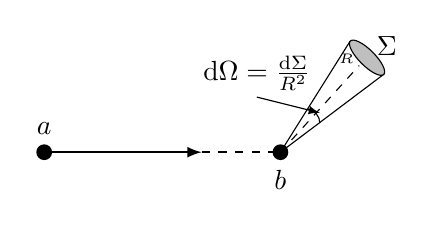
\begin{tikzpicture}

% Puntos iniciales
\fill[black] (-2,0)  circle (0.1);
\node[above] at (-2,0.1) {$a$};

% Flechas y líneas
\draw[-latex, thick] (-2,0)--(0,0);
\draw[dashed, thick] (0,0)--(1,0);
\fill[black] (1,0)  circle (0.1);
\node[below] at (1,-0.1) {$b$};

% Líneas delgadas que forman el ángulo
\draw[] (1,0)--(1.885,1.41);
\draw[] (1,0)--(2.32,0.995);
\draw[dashed] (1,0)--(2,1.1);
\node[above left] at(2.05,1){\tiny{$R$}};
\node[above right] at(2.1,1.1){$\Sigma$};
%Elipse
\draw[rotate around={-45:(2.1,1.2)}, fill=lightgray] (2.1,1.2)ellipse (0.3 and 0.1);
     \draw (1.5,0.37) arc[start angle=0, end angle=80, radius=0.18];

\node at(0.7,1){$\dd \Omega=\frac{\dd \Sigma}{R^2}$};
\draw[-latex] (0.7,0.7)--(1.5,0.5);
\end{tikzpicture}
\end{document}


